\documentclass[12pt, oneside, titlepage]{article}   	% use "amsart" instead of "article" for AMSLaTeX format

\usepackage{graphicx}
\graphicspath{ {\string} }
\usepackage{subcaption}

%%%%%%%%%%%%%%%%%%%%%%%%%%%%%%%%%%%%%%%%%%%%%%%%%%%%
% set up packages
%%%%%%%%%%%%%%%%%%%%%%%%%%%%%%%%%%%%%%%%%%%%%%%%%%%%
\usepackage{geometry}                
\usepackage{textcomp}                
\usepackage{amsmath}                
\usepackage{graphicx}                
\usepackage{amssymb}                
\usepackage{fancyhdr}                
\usepackage{subcaption}                
\usepackage{bm}                
% \usepackage{lineno}
% package for comments
\usepackage{soul}

\usepackage[breaklinks=true]{hyperref}

\usepackage[superscript,noadjust]{cite} % puts dash in citations to abbreviate
\usepackage [autostyle, english = american]{csquotes} % sets US-style quotes

\usepackage{etoolbox} % block quotes

\usepackage{float}
\usepackage{color}

\usepackage{pgf}
\usepackage{tikz}
\usepackage{eqnarray}

\usepackage{listings} % code blocks
\usepackage{setspace}

\usepackage{lscape}

% tikz background
\usetikzlibrary{backgrounds, fit}


\usepackage{natbib}
%\bibliographystyle{abbrvnat}
\setcitestyle{authoryear,open={(},close={)}}

\usepackage{pdfpages}


%%%%%%%%%%%%%%%%%%%%%%%%%%%%%%%%%%%%%%%%%%%%%%%%%%%%
% call packages
%%%%%%%%%%%%%%%%%%%%%%%%%%%%%%%%%%%%%%%%%%%%%%%%%%%%	
\geometry{letterpaper, marginparwidth=60pt} % sets up geometry              		
% \linenumbers % adds line numbers 
\MakeOuterQuote{"} % sets quote style
\doublespacing % setspace

%%%%%%%%%%%%%%%%%%%%%%%%%%%%%%%%%%%%%%%%%%%%%%%%%%%%
% patches with etoolbox 
%%%%%%%%%%%%%%%%%%%%%%%%%%%%%%%%%%%%%%%%%%%%%%%%%%%%	
% block quotes
\AtBeginEnvironment{quote}{\small}

% linenumbers
%\makeatletter
%\patchcmd{\@startsection}{\@ifstar}{\nolinenumbers\@ifstar}{}{}
%\patchcmd{\@xsect}{\ignorespaces}{\linenumbers\ignorespaces}{}{}
% \makeatother

%%%%%%%%%%%%%%%%%%%%%%%%%%%%%%%%%%%%%%%%%%%%%%%%%%%%
% tikzlibrary modifications
%%%%%%%%%%%%%%%%%%%%%%%%%%%%%%%%%%%%%%%%%%%%%%%%%%%%	
\usetikzlibrary{fit}
\usetikzlibrary{positioning}
\usetikzlibrary{arrows}
\usetikzlibrary{automata}

%%%%%%%%%%%%%%%%%%%%%%%%%%%%%%%%%%%%%%%%%%%%%%%%%%%%
% page formatting; exact 1 in margins
%%%%%%%%%%%%%%%%%%%%%%%%%%%%%%%%%%%%%%%%%%%%%%%%%%%%
\pagestyle{plain}                                                     

\setlength{\textwidth}{6.5in}    
\setlength{\oddsidemargin}{0in}
\setlength{\evensidemargin}{0in}
\setlength{\textheight}{8.5in}
\setlength{\topmargin}{0in}
\setlength{\headheight}{0in}
\setlength{\headsep}{0in}
\setlength{\footskip}{.5in}

%%%%%%%%%%%%%%%%%%%%%%%%%%%%%%%%%%%%%%%%%%%%%%%%%%%%
% defining code blocks using listings package
%%%%%%%%%%%%%%%%%%%%%%%%%%%%%%%%%%%%%%%%%%%%%%%%%%%%

\definecolor{dkgreen}{rgb}{0,0.6,0}
\definecolor{gray}{rgb}{0.5,0.5,0.5}
\definecolor{mauve}{rgb}{0.58,0,0.82}

\lstset{frame=tb,
  language=R,
  aboveskip=3mm,
  belowskip=3mm,
  showstringspaces=false,
  columns=flexible,
  basicstyle={\small\ttfamily},
  numbers=none,
  numberstyle=\tiny\color{gray},
 % keywordstyle=\color{blue},
  commentstyle=\color{dkgreen},
  stringstyle=\color{mauve},
  breaklines=true,
  breakatwhitespace=true,
  tabsize=3,
  otherkeywords={0,1,2,3,4,5,6,7,8,9},
  deletekeywords={data,frame,length,as,character,dunif,ps},
}

%%%%%%%%%%%%%%%%%%%%%%%%%%%%%%%%%%%%%%%%%%%%%%%%%%%%
%%%%%%%%%%%%%%%%%%%%%%%%%%%%%%%%%%%%%%%%%%%%%%%%%%%%
% begin document
%%%%%%%%%%%%%%%%%%%%%%%%%%%%%%%%%%%%%%%%%%%%%%%%%%%%
%%%%%%%%%%%%%%%%%%%%%%%%%%%%%%%%%%%%%%%%%%%%%%%%%%%%

\begin{document}

\subsection*{Our problem}

We write per capita reproductive success as the product of seedling survival to fruiting, fruits per plant, and seeds per fruit (all per capita):
%
\begin{align}
  \begin{split}
\mathrm{per\ capita\ RS} & =  \sigma F \phi
  \end{split}
\end{align}

We want to understand the contribution of variance in each component of reproductive success to the overall variance in reproductive success. 

\subsection*{Background}

Venable 2007 calculates the "risk associated with germination\dots as the geometric standard deviation of per capita reproductive success." In that paper, the geometric standard deviation of per capita reproductive success is expressed as:
%
\begin{align}
  \begin{split}
\mathrm{geometric\ SD(per\ capita\ RS)} = \exp \big( SD( \mathrm{ln} (\mathrm{per\ capita\ RS} ) ) \big)
  \end{split}
\end{align}

That's what I've used to calculate the standard deviation in per capita reproductive success so far. When I was thinking and reading about how to decompose the variance of per capita reproductive success, I learned that this expression for the geometric standard deviation is derived from a result involving the log-normal distribution (Kirkwood 1979). I had to learn a bit more about this to figure out how/whether I could decompose the variance for this. In the rest of this, I give the geometric mean, geometric variance, and geometric standard deviation (de Carvalho 2016).  I then write out what I think should be the geometric covariance, but note that I have not found a good reference for the expression.

\clearpage
\newpage

\subsection*{Geometric mean}

The geometric mean $\mu_g$ of ${x_1, x_2, \dots, x_n}$ is:
%
\begin{align}
  \begin{split}
& \mu_g = ( x_1 x_2 \dots x_n )^{1/n} \\
& \ln ( \mu_g ) = \frac{1}{n}  \ln ( x_1 x_2 \dots x_n ) 
  \end{split}
\end{align}

We can rewrite this to show that the log of the geometric mean is equal to the arithmetic mean of the logs:
%
\begin{align}
  \begin{split}
\ln ( \mu_g )  & = \frac{1}{n}  \big( \ln ( x_1 ) +  \ln ( x_2  ) +  \dots + \ln ( x_n ) \big)
\\ \ln ( \mu_g ) & =  \frac{1}{n}  \sum\limits_{i=i}^n \ln ( x_i) 
\\  \mu_g   & =  \exp \Big( \frac{1}{n} \sum\limits_{i=i}^n \ln ( x_i)  \Big)
  \end{split}
\end{align}

\subsection*{Geometric variance}

The log of the geometric variance is equal to the arithmetic variance of the logs of ${x_1, x_2, \dots, x_n}$:
%
\begin{align}
  \begin{split}
\ln ( \sigma^2_g )  & =  \frac{ 1} { n - 1 } \sum\limits_{i=i}^n \big( \ln x_i - \ln \mu_g \big)^2  
  \end{split}
\end{align}

We use the geometric mean $\mu_g$ to calculate the geometric variance: 
%
\begin{align}
  \begin{split}
\mathrm{geometric\ Var(}\bm{x}\mathrm{)} & = \exp \frac{\sum\limits_{i=i}^n \big( \ln x_i - \ln \mu_g \big)^2 } { n - 1 }
\\ & =  \exp \frac{\sum\limits_{i=i}^n \big( \ln \frac{x_i}{\mu_g} \big)^2 } { n - 1 }
  \end{split}
\end{align}

% https://quant.stackexchange.com/questions/25371/geometric-means-standard-deviation-and-sharpe-ratios

\subsection*{Geometric standard deviation}

The log of the geometric standard deviation is equal to the arithmetic standard deviation of the logs of ${x_1, x_2, \dots, x_n}$:
%
\begin{align}
  \begin{split}
\ln ( \sigma_g )  & = \sqrt{ \frac{ 1} {n - 1} \sum\limits_{i=i}^n \big( \ln x_i - \ln \mu_g \big)^2  }
  \end{split}
\end{align}

We use the geometric mean $\mu_g$ to calculate the geometric standard deviation: 
%
\begin{align}
  \begin{split}
\mathrm{geometric\ SD(}\bm{x}\mathrm{)} & = \exp \sqrt{ \frac{\sum\limits_{i=i}^n \big( \ln x_i - \ln \mu_g \big)^2 } { n - 1 }}
\\ & = \exp \sqrt{ \frac{\sum\limits_{i=i}^n \big( \ln \frac{x_i}{\mu_g} \big)^2 } { n - 1 }}
  \end{split}
\end{align}

\subsection*{Geometric co-variance}

I have not been able to find a reference for this expression. But I think that by extension, the log of the geometric covariance is equal to the arithmetic covariance of the logs of ${x_1, x_2, \dots, x_n}$ and ${y_1, y_2, \dots, y_n}$:
%
\begin{align}
  \begin{split}
\ln  cov(\bm{x},\bm{y} ) = \frac{1 }{ n - 1 } \sum\limits_{i=i}^n \big( \ln x_i - \ln \mu_{x,g} \big) \times  \big( \ln y_i - \ln \mu_{y,g} \big) 
  \end{split}
\end{align}

We use the geometric means $\mu_{x,g}$ of $\bm{x}$ and $\mu_{y,g}$ of $\bm{y}$to calculate the geometric standard deviation: 
%
\begin{align}
  \begin{split}
\mathrm{geometric\ Cov(}\bm{x,y}\mathrm{)} & = \exp \frac{\sum\limits_{i=i}^n \big( \ln \frac{x_i}{\mu_{x,g}} \big) \times \big( \ln \frac{y_i}{\mu_{y,g} }  \big) } { n - 1 } 
\\ & = \exp \frac{\sum\limits_{i=i}^n \big( \ln x_i - \ln \mu_{x,g} \big) \times  \big( \ln y_i - \ln \mu_{y,g} \big) } { n - 1 }
  \end{split}
\end{align}

\subsection*{Variance decomposition}

The arithmetic variance of the sum of random variables is the sum of the variance of each random variable plus two times the covariance of the random variables. The variance and covariance terms are additive. The arithmetic variance of the sum of random variables $X$ and $Y$ is written as:
%
\begin{align}
  \begin{split}
\mathrm{Var}(X + Y) = \mathrm{Var}(X) + \mathrm{Var}(Y) + 2 \mathrm{Cov} (X, Y)
  \end{split}
\end{align}

I think the log of the geometric variance of the sum of random variables $X$ and $Y$ should be the following. Here I use $\sigma$ to denote the arithmetic variance and $\sigma_g^2$ to denote the geometric variance:
%
\begin{align}
  \begin{split}
\ln \big( \sigma_g^2( X + Y) \big) = \sigma^2( \ln X) + \sigma^2(\ln Y) + 2 \times \mathrm{geom\ cov} (\ln X, \ln Y)
  \end{split}
\end{align}

The geometric variance of the sum of random variables is multiplicative. I think this shows up when rewriting the equation above. 
%
\begin{align}
  \begin{split}
\ln \big( \sigma_g^2( X + Y) \big) & = \sigma^2( \ln X) + \sigma^2(\ln Y) + 2 \times \mathrm{ cov} (\ln X, \ln Y) \\
 \sigma_g^2( X + Y) & = \exp \big( \sigma^2( \ln X) + \sigma^2(\ln Y) + 2 \times \mathrm{ cov} (\ln X, \ln Y) \big) \\
 & = \exp \big( \sigma^2( \ln X) \big) \exp \big(  \sigma^2(\ln Y) \big) \exp \big(  2 \times \mathrm{ cov} (\ln X, \ln Y) \big) \\
 & = \exp \big( \sigma^2( \ln X) \big) \exp \big(  \sigma^2(\ln Y) \big)  \big( \exp \mathrm{ cov} (\ln X, \ln Y) \big) ^2
  \end{split}
\end{align}

In the last line of the equation above, there are some familiar terms: the geometric variance of X, the geometric variance of Y, and the geometric covariance of X and Y (which is squared rather than multiplied by two).

\subsection*{Back to our problem}

We want to understand the contribution of variance in each component of reproductive success to the overall variance in reproductive success. The log of the geometric variance of a quantity is the arithmetic variance of the log of that quantity. If reproductive success is a product of three terms, the log of the geometric variance of reproductive success is the arithmetic variance of the log of the product of those terms. 
%
\begin{align}
  \begin{split}
\mathrm{geometric\ var(per\ capita\ RS)} & = \exp \big( \mathrm{Var}( \ln ( \sigma F \phi) ) \big) 
 \\ & = \exp \big(  \mathrm{Var}( \ln ( \sigma ) + \ln ( F ) + \ln ( \phi) ) \big) 
  \end{split}
\end{align}

Using the properties of logarithms lets us rewrite this more, so that we can see that it is the arithmetic variance of the sum of the logs. We can then apply what we know about the properties of variances and exponents (as above) to expand the expression.
%
\begin{align}
  \begin{split}
\mathrm{geometric\ var(per\ capita\ RS)}  = e^{\mathrm{Var}( \ln \sigma ) } e^{\mathrm{Var}( \ln F ) }  e^{\mathrm{Var}( \ln \phi ) } (e^{\mathrm{Cov}( \ln \sigma, \ln F ) })^2  (e^{\mathrm{Cov}( \ln \sigma, \ln \phi ) })^2  (e^{\mathrm{Cov}( \ln F, \ln \phi ) })^2
  \end{split}
\end{align}

I've verified that this expression returns the correct result by comparing the geometric variance calculated from the values for reproductive success and plotting them against the product of the decomposed terms (see Figure 1).

Interpretation of the decomposition is different than for an arithmetic variance. I'm not sure I have the nuances but here is what I have so far. First, the variance has a minimum value of 1 because of the exponents. This corresponds to an arithmetic variance of 0. Second, covariances have a minimum of 0. Values of 1 for the covariance indicate a lack of covariation; values less than 1 indicate negative covariation; values greater than one indicate positive covariation. I'm not sure how to plot these results because the contributions are multiplicative but I've tried a few things. 

First, it seems like the geometric variance in sigma is much larger than any other terms for many sites (see Figure 2). Fecundity has the next highest variance, and then phi. The covariances are mostly positive, though there does seem to be both positive and negative covariances for sigma and fecundity.

Second, the sites vary in how their variances are distributed but some patterns emerge from plotting each sites components individually. Variance in seedling survival to fruiting dominates the other components at roughly half the sites. The other sites see other patterns such as a more even distribution of variances (e.g. Camp 3), equal variance in seedling survival to fruiting and fruits per plant (Lucas Creek West), or decreasing variance when moving from survival to fruits to seeds (e.g. Upper Richbar).

I've included the plots for interannual estimates of seedling survival to fruiting, total fruit per plant equivalents, and seeds per fruit. Looking at those, it seems like high variance in seedling survival to fruiting may be the result of sites with year(s) of very low seedling survival to fruiting. Mill Creek saw three years with survival very close to zero.



 \begin{figure}[h]
   \centering
       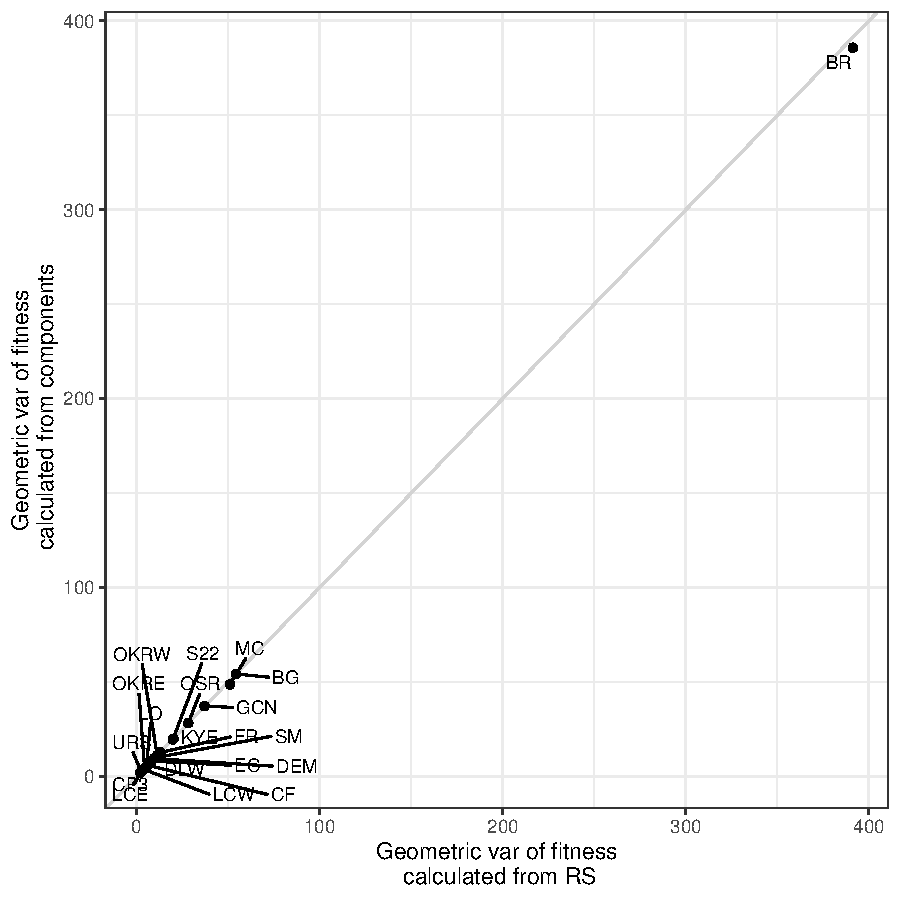
\includegraphics[page=1,width=1\textwidth]{../../figures/appendix/varianceDecomp/comparison.pdf}  
    \caption{ Compares the geometric variance calculated from the values for reproductive success with the product of the decomposed terms. }
 \label{fig:test}
\end{figure}

% See pages 270 in Caswell

 \begin{figure}[h]
   \centering
       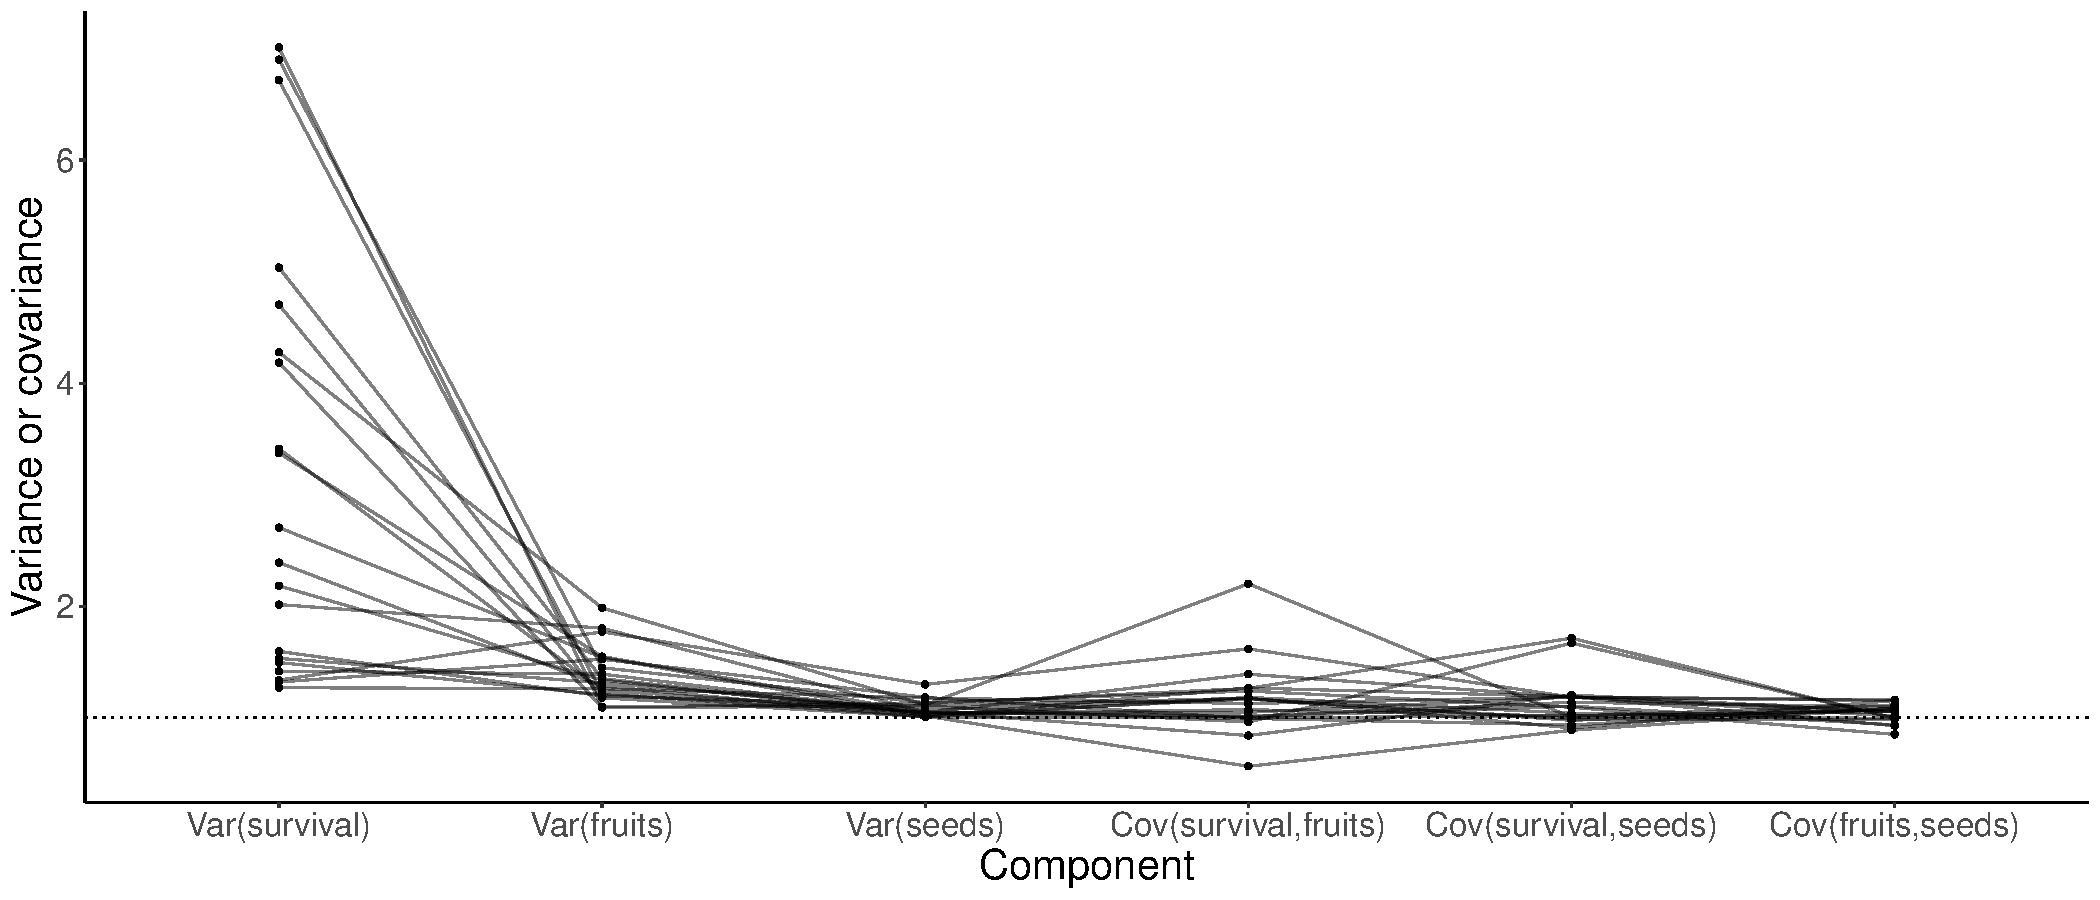
\includegraphics[page=1,width=1\textwidth]{../../figures/appendix/varianceDecomp/lineplot.pdf}  
    \caption{ Plots the variance and covariance terms. The covariance terms have not been squared here, as they would be in the contribution to reproductive success - not sure if that's something I need to do? }
 \label{fig:test}
\end{figure}

% DOES IT MAKE SENSE HERE TO SHOW 2*COVARIANCE TERM?
% TO UNDERSTAND THEIR CONTRIBUTION RELATIVE TO THE VARIANCE TERMS

%\begin{landscape}
 \begin{figure}[h]
   \centering
       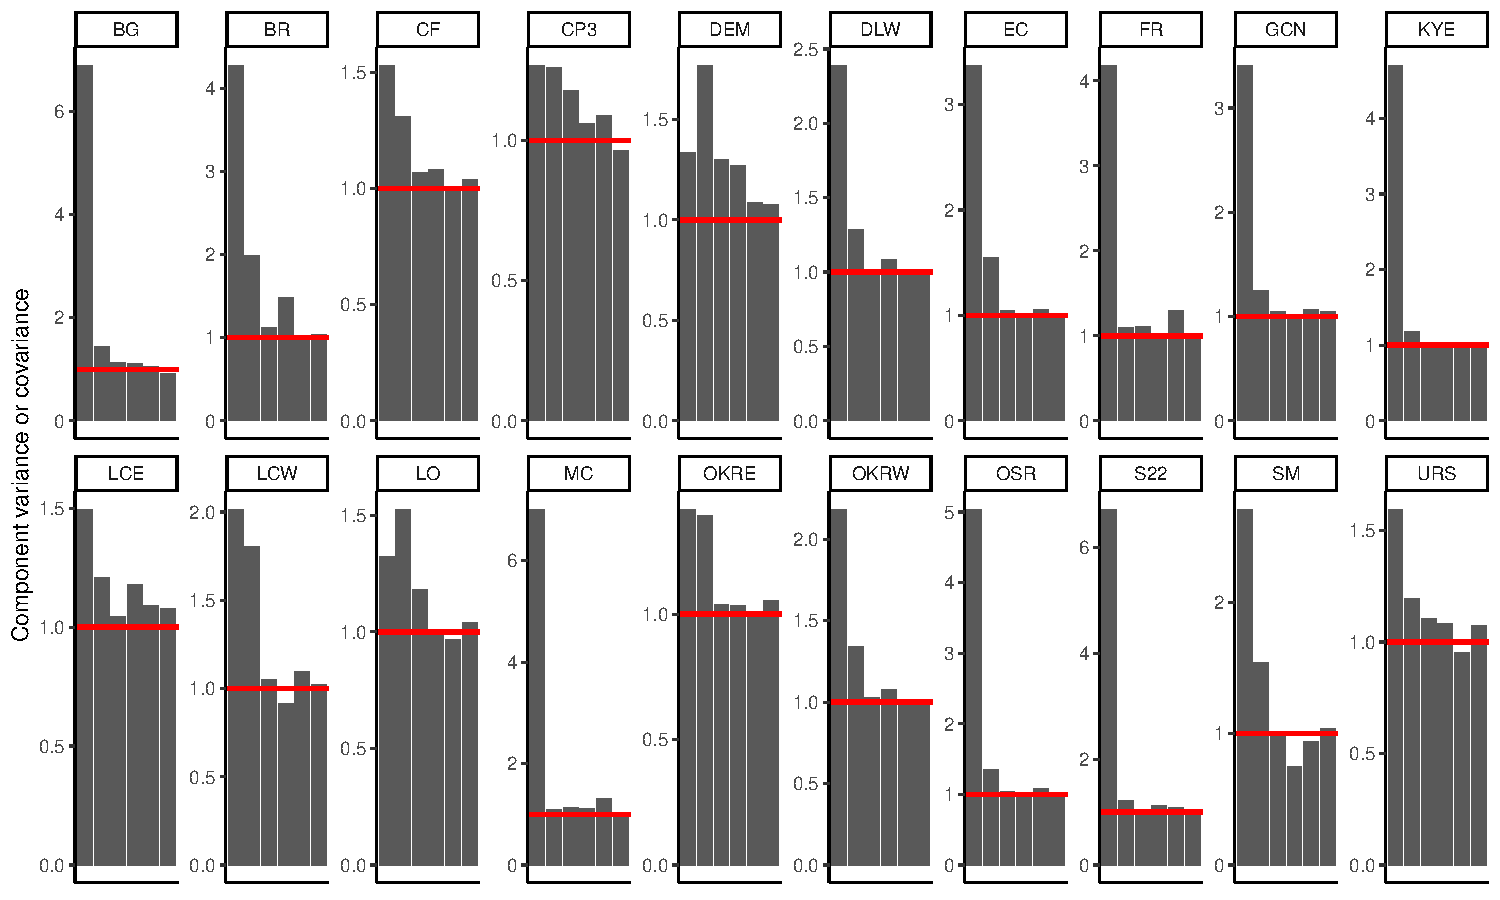
\includegraphics[page=1,width=1\textwidth]{../../figures/appendix/varianceDecomp/barPlots.pdf}  
    \caption{ Plots the variance and covariance terms for each site. The covariance terms have not been squared here, as they would be in the contribution to reproductive success - not sure if that's something I need to do? The bars are arranged in the same order as in the previous figure: Var(sigma), Var(F), Var(phi), Cov(sigma,F), Cov(sigma,phi), Cov(F,phi). The y-axis scales vary for each plot so I have included a red line at 1; this is the minimum for the variance terms and the value when there is no covariance.  }
 \label{fig:test}
\end{figure}
%\end{landscape}

\newpage
\clearpage

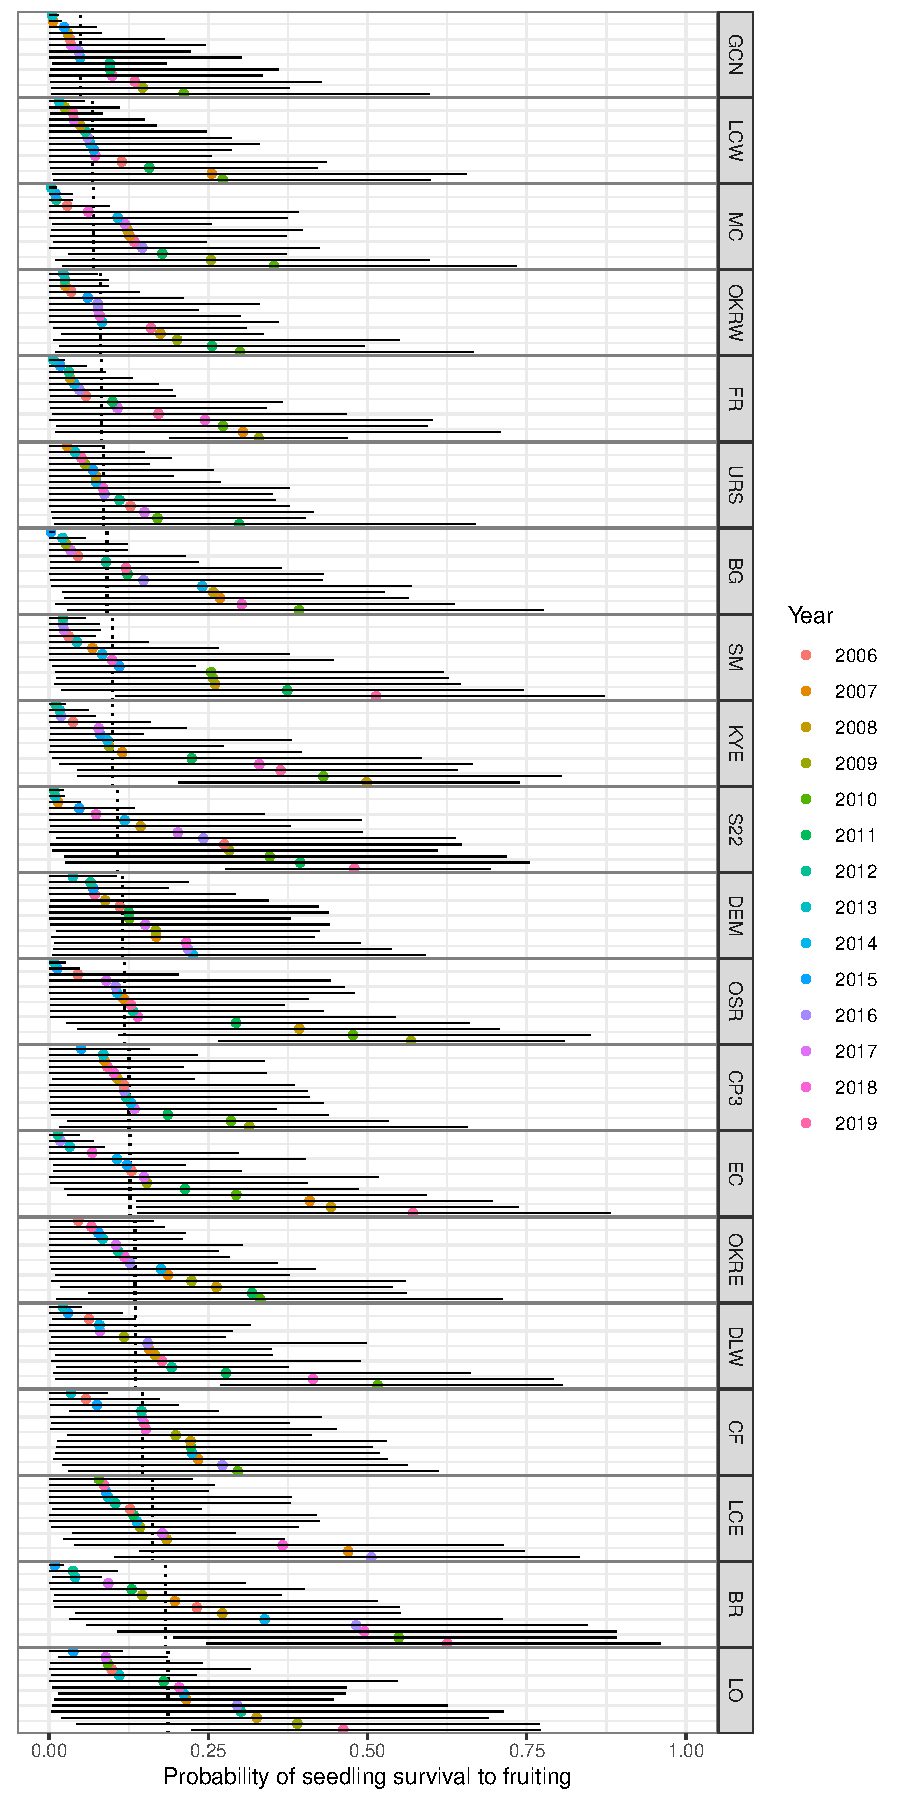
\includepdf[pages=-]{../../figures/interannualSigma.pdf}
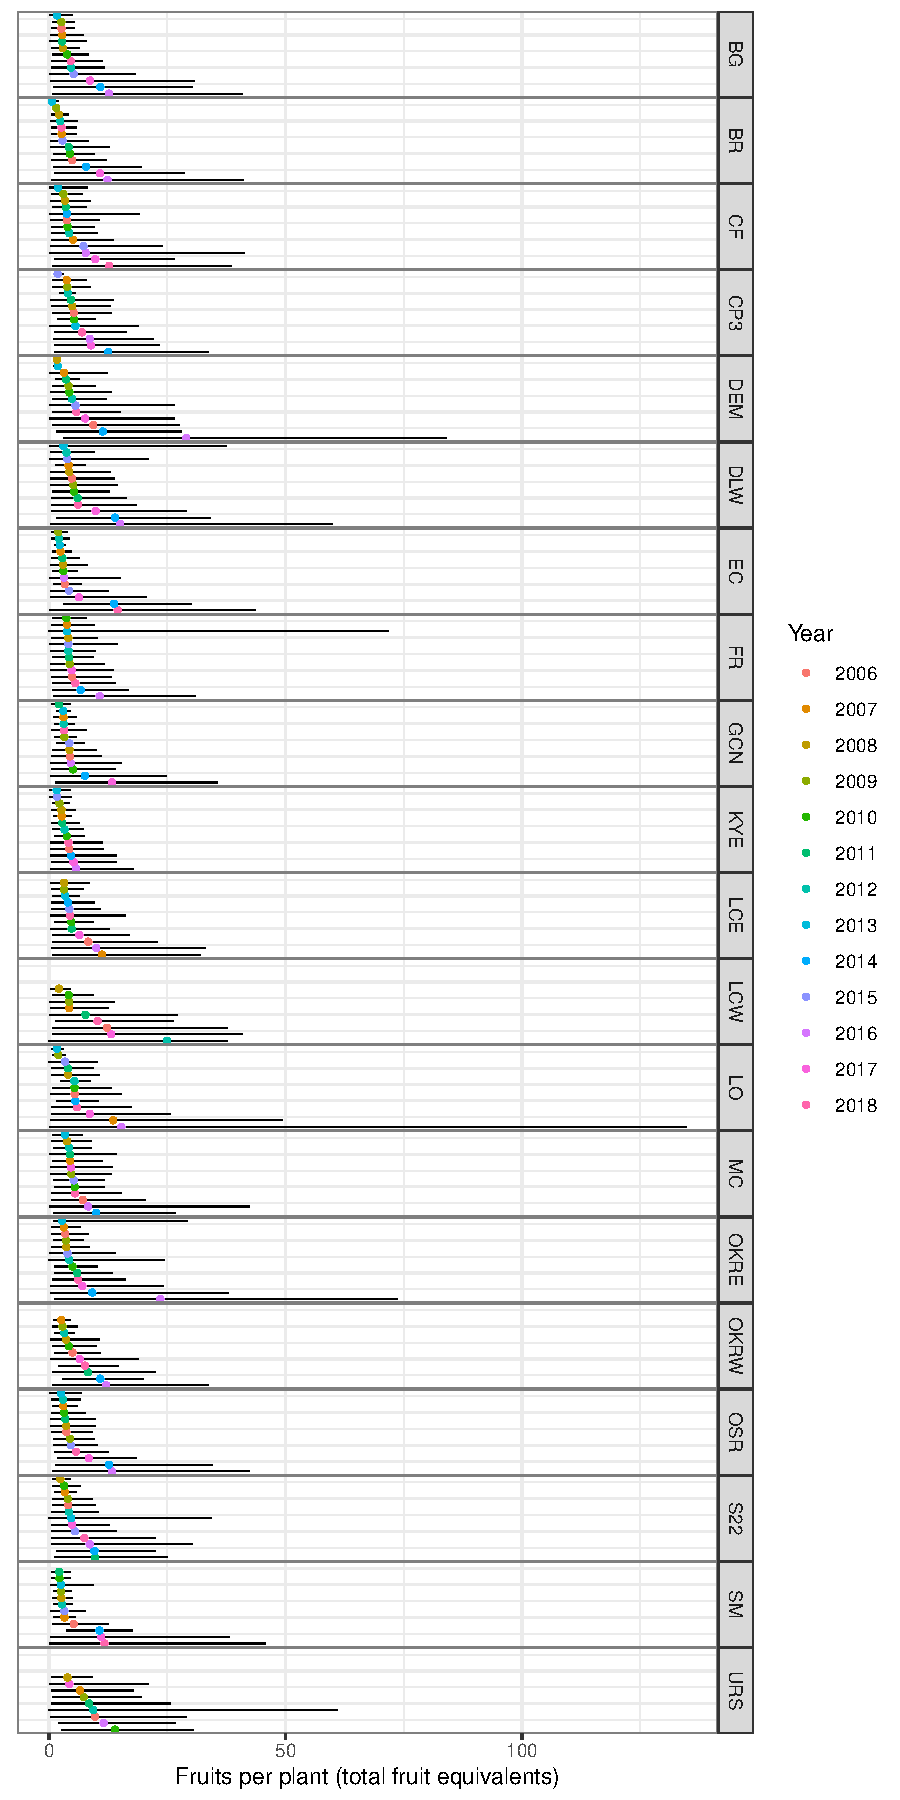
\includepdf[pages=-]{../../figures/interannualTFEFull.pdf}
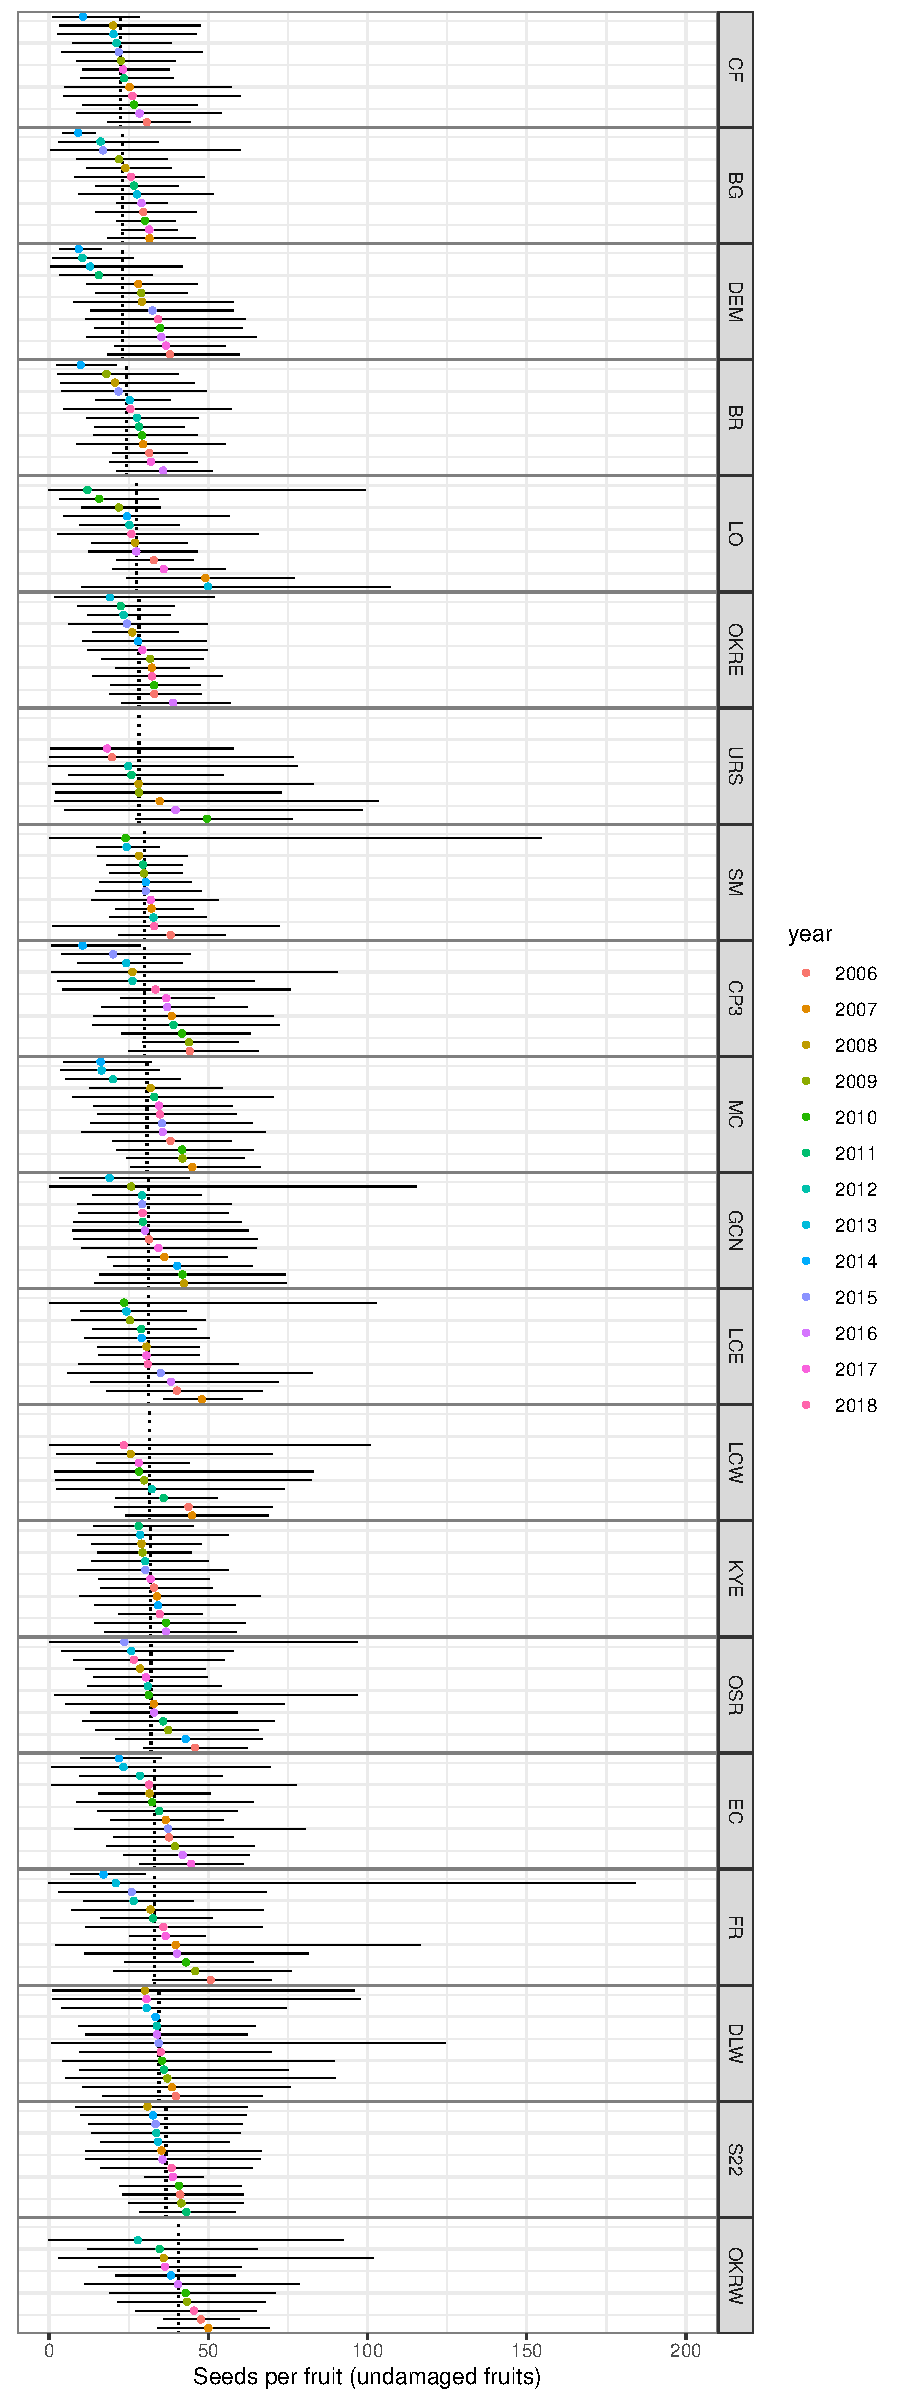
\includepdf[pages=-]{../../figures/interannualSeeds.pdf}



\end{document}
